\section{Funktionsweise Yamaha Electron D80}
\label{sec:d80}

Im folgenden Abschnitt wird der ursprüngliche Aufbau der Rhythmus-Sektion der Yamaha Electron D80 betrachtet, der für unser Projekt genutzt wurde.

\begin{figure}[H]
    \centering
    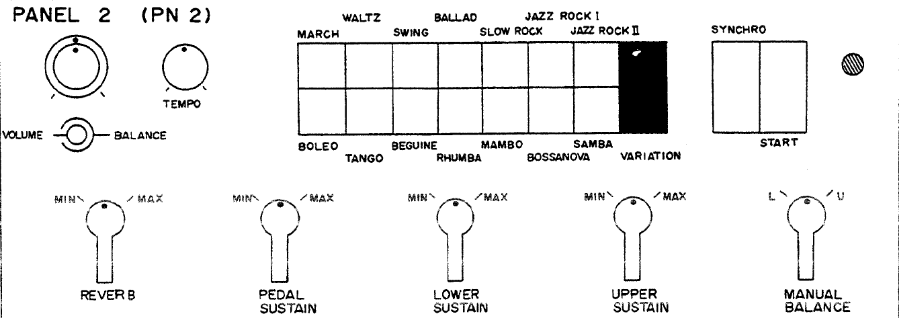
\includegraphics[width=0.8\textwidth]{Images/Rhythmus.png}
    \caption[Bedieneroberfläche]{Bedieneroberfläche \cite{ServiceManual}}
    \label{fig:Bediener Oberfläche}
\end{figure}

Auf dem beigefügten Bild ist die Bedienoberfläche der Rhythmus-Sektion zu sehen. Deutlich erkennbar sind die 14 verfügbaren Rhythmusvariationen, die durch das Drücken der entsprechenden Tasten ausgewählt werden können. Beim Betätigen einer dieser Tasten erklingt das zugehörige Rhythmusmuster.

Im Hintergrund wird der Integrierte Schaltkreis des Chips YM22800 getriggert. Dieser dient als logische Schaltung, die die verschiedenen Schaltkreise zur Klangerzeugung in bestimmter Reihenfolge ansteuert. Diese Funktionsweise ist im folgenden Ausschnitt aus dem Schaltplan ersichtlich.

An dieser Stelle sei darauf hingewiesen, dass wir in unserem Projekt die Ansteuerung mithilfe eines programmierbaren Mikrocontrollers realisiert haben, was es uns ermöglicht, beliebige Rhythmusmuster zu realisieren. Eine ausführlichere Erläuterung dazu erfolgt in Abschnitt \ref{midi-hardwareentwurf}.


\begin{figure}[H]
    \centering
    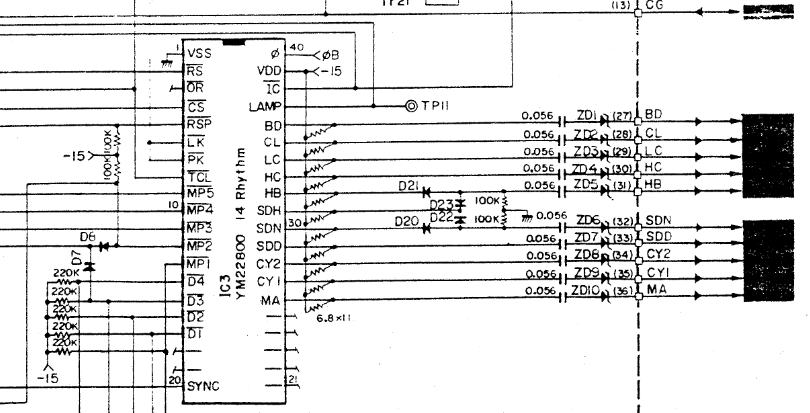
\includegraphics[width=0.7\textwidth]{Images/YM22800.png}
    \caption[YM22800]{YM22800 \cite{ServiceManual}}
    
    \label{fig:YM22800}
\end{figure}

Wie zuvor beschrieben, werden die Impulse an die jeweiligen Schaltungen zur Klangerzeugung weitergeleitet. Das nachfolgende Bild dient dazu, die Komplexität zu veranschaulichen, ohne jedoch auf die Details der Schaltung einzugehen, die im nächsten Abschnitt genauer erläutert werden.

\begin{figure}[H]
    \centering
    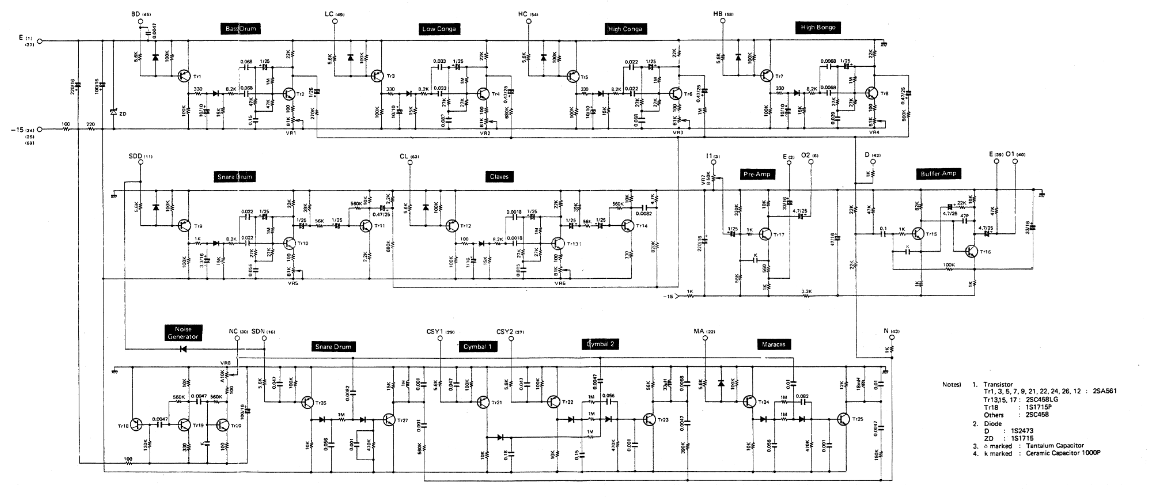
\includegraphics[width=1\textwidth]{Images/RC.png}
    \caption[Klangerzeugung Schaltplan]{Klangerzeugung Schaltplan \cite{ServiceManual}}
    
    \label{fig:Klangerzeugung Schaltplan}
\end{figure}
